\section{Resource Management with RL}

% ---------------------------------------------------------------- Slide 42
\begin{frame}{Resource Management with RL}
\vfill
\centering
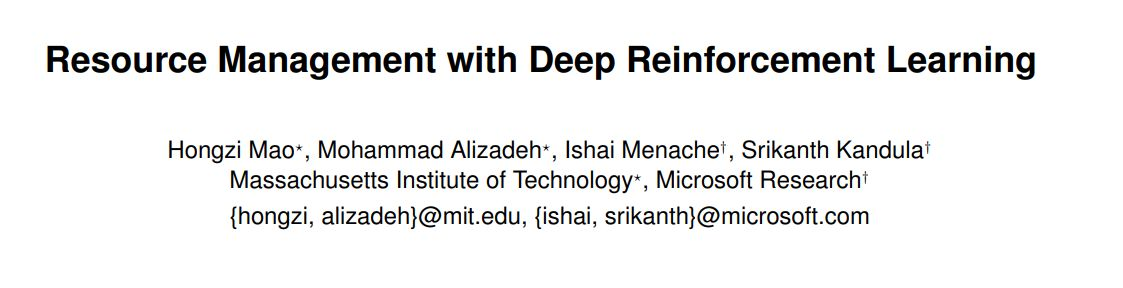
\includegraphics[width=0.96\linewidth,keepaspectratio]{images/rl-real-world/figures/resource-diagram.jpg}%
\footnote[0]{\scriptsize Mao et al. \href{https://people.csail.mit.edu/alizadeh/papers/deeprm-hotnets16.pdf}{Resource Management with Deep Reinforcement Learning}.}
\vfill
\end{frame}

% ---------------------------------------------------------------- Slide 43
\begin{frame}{Resource Management with RL}
\begin{itemize}
    \item Resource Management is a difficult online decision making task
    \item Requires to understand the workload and environment
    \item RL solution for resource management!
\end{itemize}
\end{frame}

% ---------------------------------------------------------------- Slide 44
\begin{frame}{Resource Management with RL}
\vfill
\centering
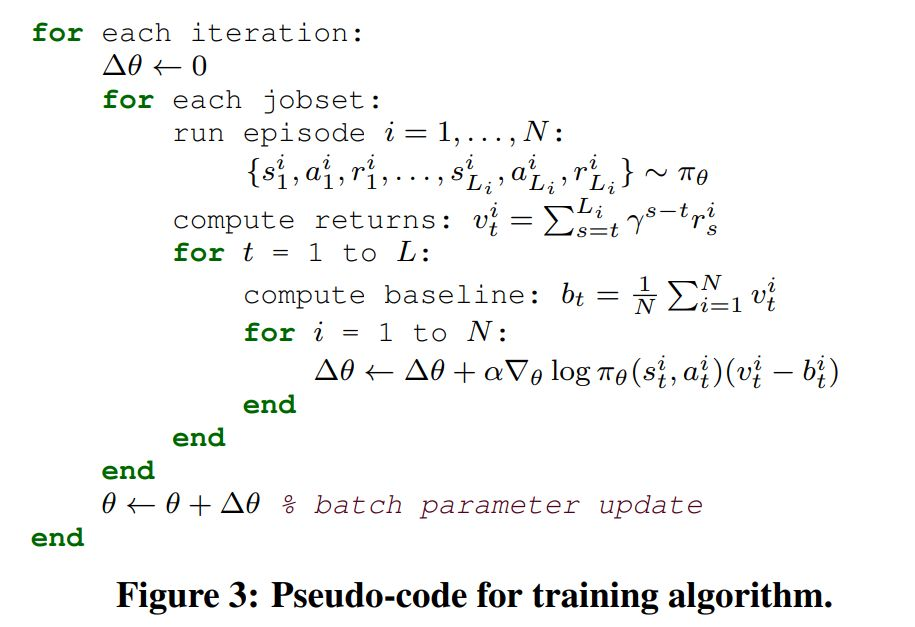
\includegraphics[width=\linewidth,height=0.80\textheight,keepaspectratio]{images/rl-real-world/figures/resource-1.jpg}
\vfill
\end{frame}

% ---------------------------------------------------------------- Slide 45
\begin{frame}{Resource Management with RL}
\vfill
\centering
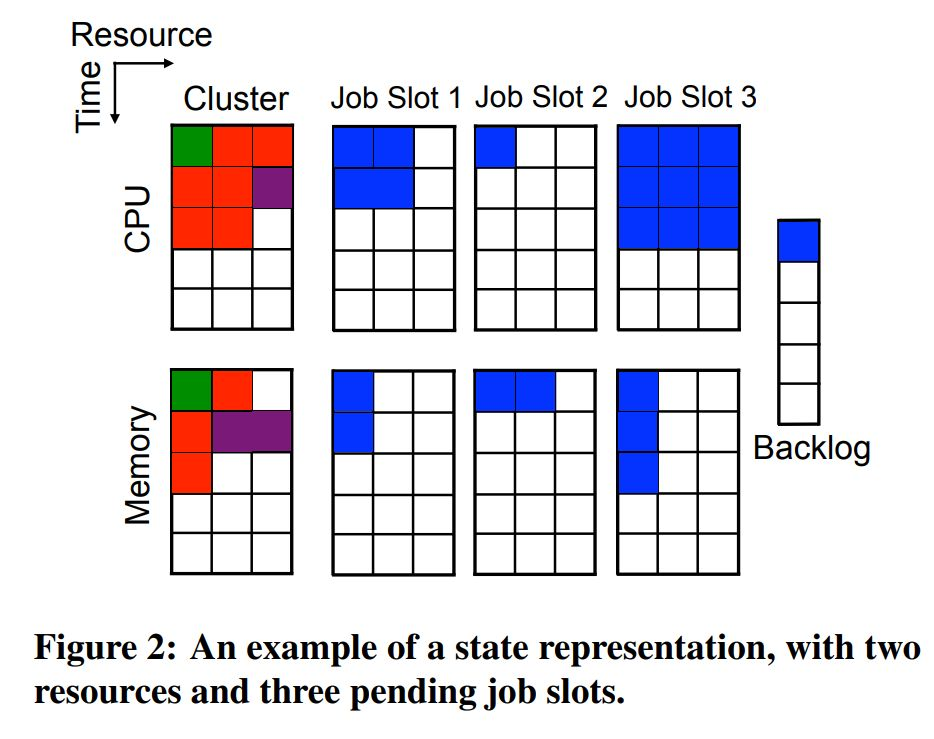
\includegraphics[width=\linewidth,height=0.82\textheight,keepaspectratio]{images/rl-real-world/figures/resource-2.jpg}
\vfill
\end{frame}

% ---------------------------------------------------------------- Slide 46
\begin{frame}{Resource Management with RL}
\vfill
\centering
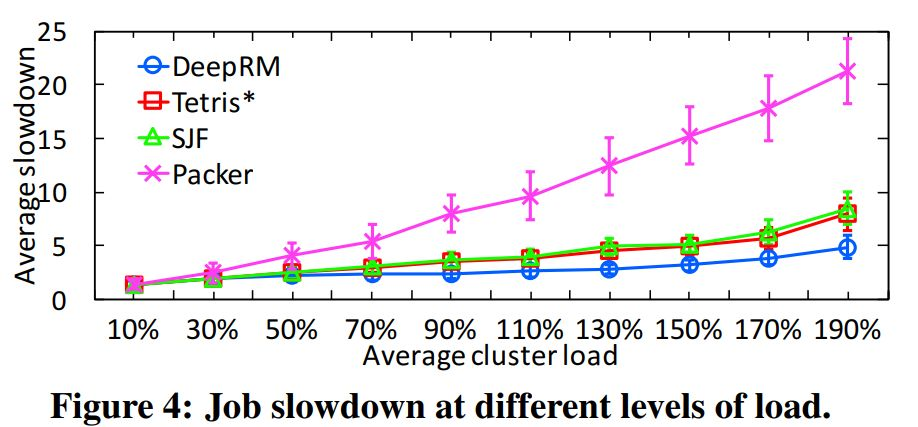
\includegraphics[width=0.8\linewidth,height=0.74\textheight,keepaspectratio]{images/rl-real-world/figures/resource-results.jpg}\\[0.3em]
{\scriptsize Figure 4: Job slowdown at different levels of load.}
\vfill
\end{frame}
